\chapter{Choice of the Kinematic Reconstruction Solution with the Smallest M($t\bar{t}$)}\label{appendix:mtt}

Only the solution of the kinematic equations \ref{alg:LS1}-\ref{alg:LS6} with minimal $m(t\bar{t})$ is taken for the further analysis.
Studies which show the advisability of this criterion were performed.

The studies were performed on the generated $t\bar{t}$ signal events. The correct solution of the kinematic equations was defined by comparing the 
solution neutrino momentum, $p_{\nu/\bar{\nu}}^{sol}$, to the generated one, $p_{\nu/\bar{\nu}}^{gen}$, with the help of a $\chi^{2}$ criterion as follows \cite{Sonnenschein:2005ed}:

\begin{equation}
 \chi^{2} = (p_{\nu_{x}}^{gen} - p_{\nu_{x}}^{sol})^{2} + (p_{\nu_{y}}^{gen} - p_{\nu_{y}}^{sol})^{2} + (p_{\nu_{z}}^{gen} - p_{\nu_{z}}^{sol})^{2} + (p_{\bar{\nu}_{x}}^{gen} - p_{\bar{\nu}_{x}}^{sol})^{2} +
 (p_{\bar{\nu}_{y}}^{gen} - p_{\bar{\nu}_{y}}^{sol})^{2} + (p_{\bar{\nu}_{z}}^{gen} - p_{\bar{\nu}_{z}}^{sol})^{2}.
\end{equation}

The fraction of correct solutions with minimal, second minimal, third minimal and fourth minimal invariant $t\bar{t}$ mass are shown in Figure \ref{fig:corrMinMtt}. In $60\%$ of 
the cases the correct solution has a minimal $m(t\bar{t})$. One might tend to average all the solutions to include always the correct solutions. However, the figures \ref{fig:Absvs}
show that the relative RMS\footnote{The relative RMS is defined as an } for the average and weighted\footnote{Wight for this study is taken according to the $m(t\bar{t})$ of the solution.} average solutions are higher then the once
of the smallest $m(t\bar{t})$.

The quality of the solution with the smallest $m(t\bar{t})$ is better then for the weighted average solution. Furthermore taking the solution with the smallest $m(t\bar{t})$ is
correct in two out of three cases while the weighted average solution can approach but never reach the correct value. Thus these studies show the advisability of selecting the
solution with the smallest $m(t\bar{t})$ for the further analysis.

\begin{figure}[t]
  \centering
  \includegraphics[width=1.2\textwidth]{/home/dolinska/Dropbox/desy_plots/Thesis/Jenya/10_appendices/KinReco/minMtt/CorrMinMtt.png}
  \caption{Fraction of correct solutions depending on the order of minimum $m(t\bar{t})$ of the solutions.}
  \label{fig:corrMinMtt}
\end{figure}

\begin{figure}[h]
\centering
\begin{subfigure}
  \centering
  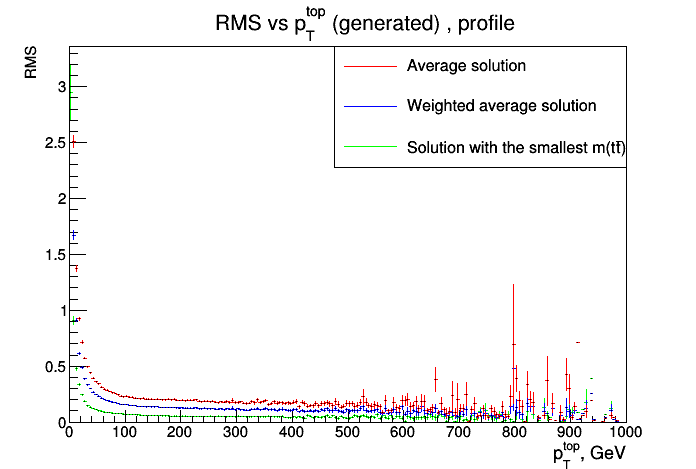
\includegraphics[width=0.6\textwidth]{10_appendices/min_Mtt/plots/Abs-pt.png}
\end{subfigure}
\begin{subfigure}
  \centering
  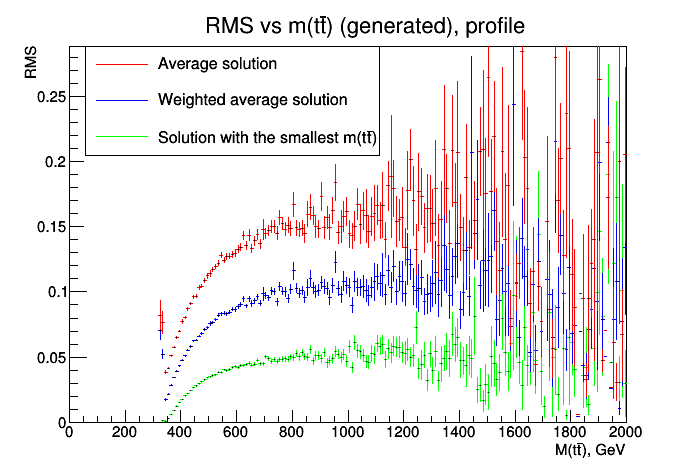
\includegraphics[width=0.6\textwidth]{10_appendices/min_Mtt/plots/Abs-mtt.png}
\end{subfigure}
\begin{subfigure}
  \centering
  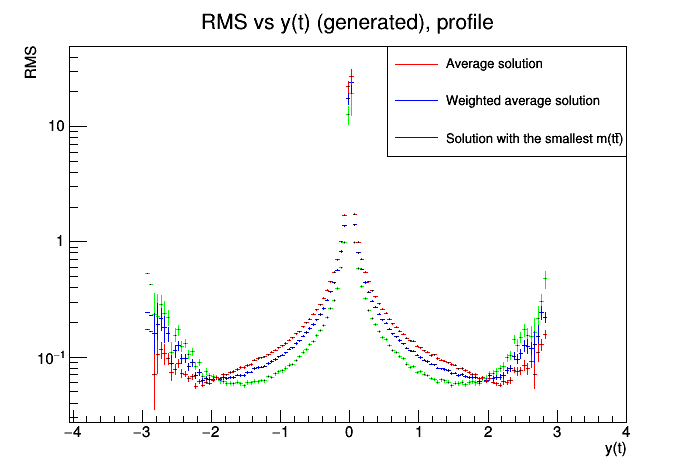
\includegraphics[width=0.6\textwidth]{10_appendices/min_Mtt/plots/Abs-y.png}
\end{subfigure}
\caption{Profile plot of the RMS relative to the top $p_{T}$ versus transverse momentum of the $t$-quark (top), invariant mass of the $t\bar{t}$ (middle) and rapidity of the
$t$-quark (bottom). The distribution for the solution of the kinematic equation with the smallest mass of the $t\bar{t}$ system is plotted as green points, the weighted average solution
as blue points and the average solution as red points.}
\label{fig:Absvs}
\end{figure}